\chapter{Introduction}

\section{Motivation}

This bachelor thesis contributes to the community-driven project ManageIQ,
a tool for cloud and virtualization services.

The main goal is to provide a new implementation for the outdated Dialog Editor
in the ManageIQ Admin and Operations User Interface while keeping in touch with
modern web 2.0 righ client interfaces.
Its current implementation is done in the interpreted programming language Ruby
and requires evaluation on the server, that is generally time consuming,
because of the need to exchange the data between user and server after almost
every user's interaction with the editor, and this forces the user to spend
an uncomfortably long amount of time in the editor.

The work on this bachelor thesis is done in collaboration with the Red Hat
company, specificaly with the CloudForms and the UX Design team.

The goal was reached by using the AngularJS JavaScript framework and several
light-weight JavaScript libraries that will be described later in the document
and the Patternfly UI framework, developed by Red Hat UX Design team.

\section{Outline}

In this thesis there will be an analysis of the implementation and
familiarization with every part related to the implementation itself.
The ManageIQ project will be described at the beginning of this document in
Chapter~\ref{ch:manageiq}.
In Chapter~\ref{ch:analysis} there will be an analysis of the current status
of the Dialog Editor.
In Chapter~\ref{ch:design} I will describe how I designed the new version
of the Dialog Editor.
Used technologies for the implementation will be described in
Chapter~\ref{ch:technologies}. Explanation of the new Dialog Editor
implementation will be in the Chapter~\ref{ch:implementation} and its
effectivity and the users comfort will be presented in
Chapter~\ref{ch:effectivity}. The results of the work will be summarized in
Chapter~\ref{ch:conclusion}.

\chapter{ManageIQ}\label{ch:manageiq}

ManageIQ is a management and automation platform that gives administrators
the possibility to simplify control of their virtual, private, and hybrid cloud
infrastructures.
Many cloud based projects, like Openstack, Amazon EC2, Google Compute Engine
or Microsoft Azure are supported by ManageIQ and that allows administrators to
manage the diverse environments by one tool.
It can automatically discover these environments wherever they are running
and bring them all under one management roof.~\cite{lwnMiq}

ManageIQ is an open source community-driven project implemented in
Ruby~on~Rails.
It is developed since 2006, when ManageIQ, Inc. was founded as a startup.
In late 2012 ManageIQ was acquired by Red~Hat to be used as the basis for the
Red~Hat CloudForms hybrid cloud management platform, and has been open-sourced
in June~2014~\cite{opensourcedMiq}.
At the time of open-sourcing ManageIQ, the dual-license GPL and Apache License
had to be used, but all the time the intention was to be single-licensed under
the Apache License exclusively.
This step was finaly achieved in March~2016 and was announced with an
explanation of the choice on the ManageIQ project
site\,\footnote{\url{https://manageiq.org/}}~\cite{licenseChange}.

All the future plans of the ManageIQ community are described in the
collaborative organization tool Trello\,\footnote{\url{https://trello.com}} and
can be discussed in many ways, mostly through IRC or discussion forums.

A part of ManageIQ is a standalone interface called the
Self Service User Interface that was introduced in Red Hat CloudForms~4.0
in December~2015\,\footnote{\url{http://cloudformsblog.redhat.com/2015/11/08/red-hat-cloudforms-4-0-public-beta-2/}}.
It is a portal allowing end users to manage their own services in a simpler
interface than ManageIQ itself~\cite{capablancaMiq}.

In the ManageIQ Admin and Operations User Interface the user can specify a
{\bf service dialog} that is used at the moment of the ordering of a service.
Also another possible usage of the service dialog is for service automation.
For such dialogs we need to have a Dialog Editor in ManageIQ Self Service
User Interface, comfortable and easy to use for end users.

Development of the ManageIQ Self Service User Interface is taking place in its
own repository, because the whole interface is a 100\% REST API driven
JavaScript application.

The source code for the ManageIQ Self Service User Interface can be found on
the web-based Git repository hosting service
GitHub\,\footnote{\url{https://github.com/ManageIQ/manageiq-ui-self\_service}}.

The reason for mentioning the Self Service User Interface in this thesis is
that this stand\-alone interface is where the new Dialog Editor will be used.

\chapter{Analysis of the current status}\label{ch:analysis}

The initial step to implementation was an investigation of the current
implementation.
There was a need to find answers for some major questions related to the
implementation, such as:
{\it``What is the Service Dialog?''},
{\it``What does the Service Dialog consist of?''} or
{\it``What are the required preferences for the Dialog?''}.

\section{Service Dialog}\label{sec:service-dialog}

In the ManageIQ interface, Service Dialogs can be found under the
{\it Automate}~$\rightarrow$~{\it Customization} tab, and there under accordion
with the label {\it Service Dialogs}.
Service Dialogs can be used in several situations. The most
common, when user wants to provision\,\footnote{obtain cloud service
ordered from a cloud service catalog} a service.
The dialog in its final form is basically an HTML form that is used to take
input from the user. This input is then passed to Automation methods.

Creating a new dialog can be divided into eight basic steps:

\begin{enumerate}
  \item Navigate to the previously mentioned tab {\it Automate}~$\rightarrow$~{\it Customization}.
  \item Select the accordion with the label {\it Service Dialog}.
  \item From the toolbar select the {\it Configuration}~$\rightarrow$~{\it Add a new Dialog} option.
  \item Fill in the information for the Dialog.
  \item Fill in the information for a Tab (or more Tabs).
  \item Fill in the information for a Box (or more Boxes).
  \item Add and configure Elements in the Boxes.
  \item Save the dialog.
\end{enumerate}

Every dialog has at least one tab that has been assigned a {\it Description}
and a {\it Label}.
The user can also choose whether the form should have a
{\it Submit} and {\it Cancel} button, as you can see in
Figure~\ref{fig:dialog-box}.

\begin{figure}[b]
  \centering
  \def\svgwidth{\columnwidth}
  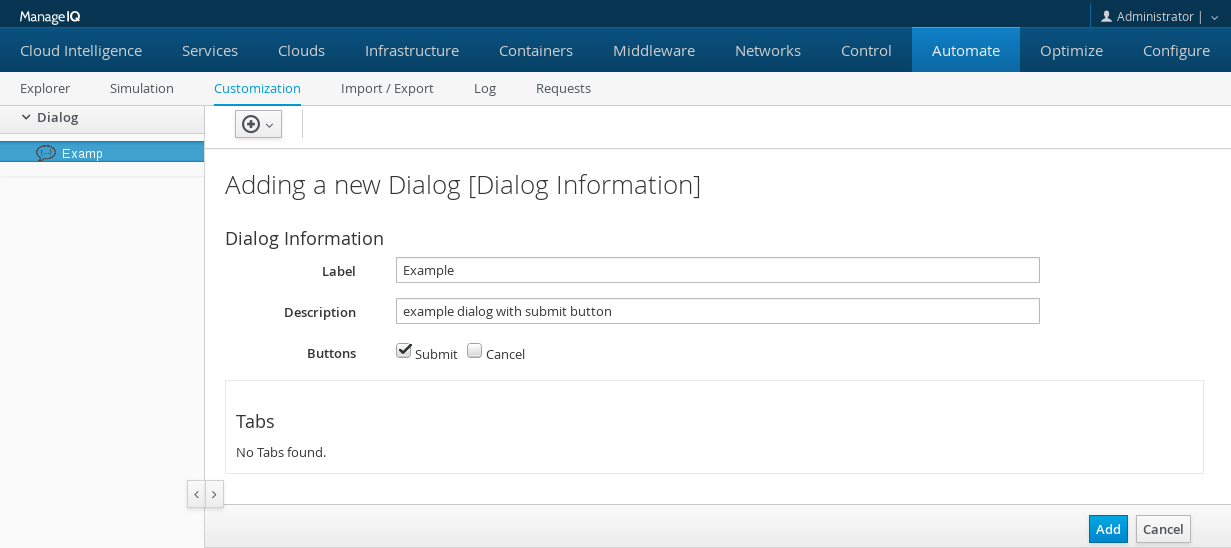
\includegraphics[width=14cm,keepaspectratio]{fig/dialog-box}
  \caption{Adding new dialog}\label{fig:dialog-box}
\end{figure}

After adding and filling in all the required information for a new tab, the
user can add a box that will be included under the tab.
The same information needs to be provided for the box.

\begin{wrapfigure}[14]{r}{60mm}
  \centering
	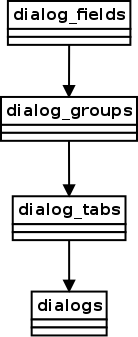
\includegraphics[width=2.5cm,keepaspectratio]{fig/dialog-scheme}
	\caption{Scheme of Dialog}\label{fig:dialog-hierarchy}
\end{wrapfigure}

A part of ManageIQ database scheme that describes tables where the dialog
content is stored can be seen in Figure~\ref{fig:dialog-hierarchy}.

After these two steps the user should be finally able to add dialog elements,
as you can see in Figure~\ref{fig:dialog-elements}.

\begin{figure}
  \centering
  \def\svgwidth{\columnwidth}
  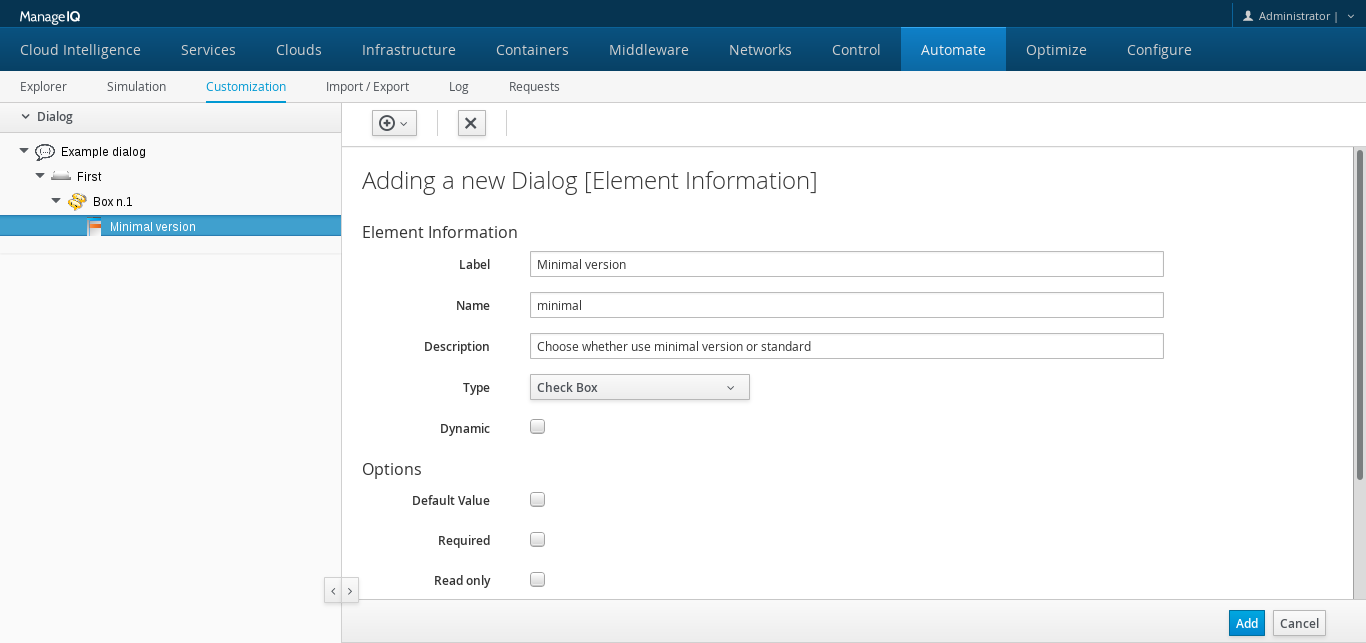
\includegraphics[width=14cm,keepaspectratio]{fig/dialog-elements}
  \caption{Adding new elements to a new dialog}\label{fig:dialog-elements}
\end{figure}

For dialogs the user has an option to choose from seven different kinds of
elements described below:

\paragraph{Text box}

Serves as an input box for text from the user. The user's ability to decide
whether the text should be obscured or not is most important for this element.
This is useful for entering passwords or any other sensitive data.

\paragraph{Text area}

Used for long texts. Compared with a Text box, a Text area does
not have the possibility to obscure the user's input.

\paragraph{Check box}

Use of a checkbox is more or less the same as of the standard HTML check boxes.
It gives the possibility to select between two values (checked or unchecked).

\paragraph{Drop down list}

Compared to the Check box, a Drop down list offers more options to choose from.
The options are presented in a drop down list.

\paragraph{Radio button}

Gives exactly the same possibilities as Drop down list, but options are
displayed using HTML radio buttons. The user has the option to choose
between a Radio button or a Drop down list, because in some cases displaying all
the possible values as options in Radio buttons may not be the most clear
solution.

\paragraph{Date control}

For every situation where the user wants to input a date, a Date control is
the most suitable option. The result is an input box where the user can
select the required date from a calendar.

\paragraph{Date time control}\label{subsub:datetime}

Offers one more option compared to Date control. It allows you to specify the
exact time of the selected day.
For every dialog it is possible to use only one Date control or
Date time control element.

\chapter{Design}\label{ch:design}

The main goal of the design was to create a single-page application for the
Dialog Editor to solve the problem of loading many pages for various elements
of the dialog.

So far the editor included many view templates for the individual steps in the
workflow of creating a dialog. That means it was necessary to load a template
for each individual steps leading to a high volume for data communication
with the server. For that reason, the Dialog Editor was designed as
a single-page application from the beginning.

The major requirement for the implementation was to simplify the current
solution. For that it was necessary to use the currently used dialog elements
described in Section~\ref{sec:service-dialog}.

Because in the process of creating the dialog, the users spend the most of
their time working with the dialog elements, it was decided that the
drag\&drop technique would be used for these components.
For that reason the toolbox containing individual elements that can be easily
dragged to the field representing the dialog content was designed.

In the initial design the toolbox was fixed to the bottom part of the page,
so it would be always visible, regardless of the size of the area filled by
the created dialog.
The only scrollable part would be the content of the dialog.
On the left side of the Figure~\ref{fig:mockup-1} there is an example of
initialized page with empty dialog. The right part of Figure~\ref{fig:mockup-1}
shows filled dialog with scrollable content.

\begin{figure}
  \centering
  \def\svgwidth{\columnwidth}
  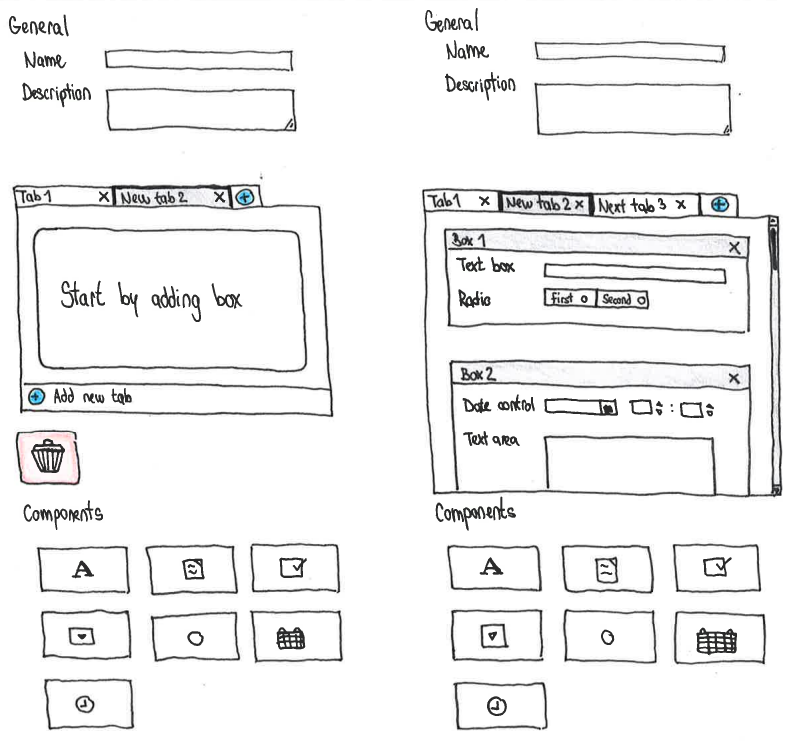
\includegraphics[width=15cm,keepaspectratio]{fig/mockup-1}
  \caption{Mockup of a first version for implementation}\label{fig:mockup-1}
\end{figure}

This initial solution was discussed with the UX Design team, that has accepted
the idea of using the toolbox, but suggested to split the page into two
vertical parts and place the toolbox to the right part of the page, as can be
seen in Figure~\ref{fig:mockup-2}.

\begin{figure}
  \centering
  \def\svgwidth{\columnwidth}
  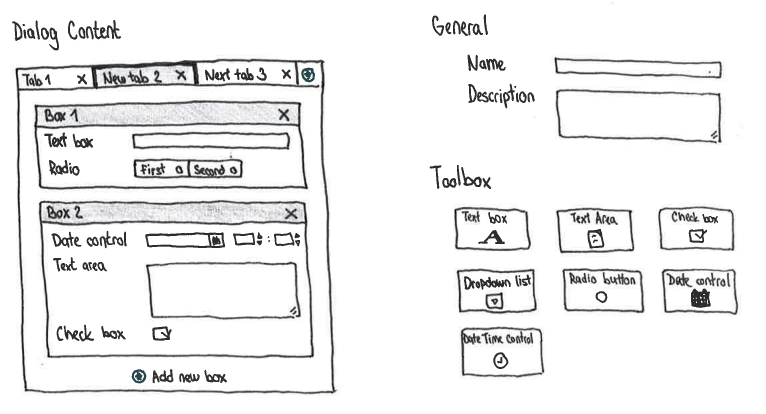
\includegraphics[width=15cm,keepaspectratio]{fig/mockup-2}
  \caption{Mockup of a second version with the toolbox on the right side of the page}
  \label{fig:mockup-2}
\end{figure}

Another option, that is still considered to be used, is to move the
elements used for creating the new tab and the new box to the toolbox in the
right part of the page. This can be seen in Figure~\ref{fig:mockup-3}.
The reason for the change is to get together all the elements that are used for
creating the dialog.
Because it is still not clear if the change will contribute to the user's
comfort, this version is still being discussed with the UX Design team.

\begin{figure}
  \centering
  \def\svgwidth{\columnwidth}
  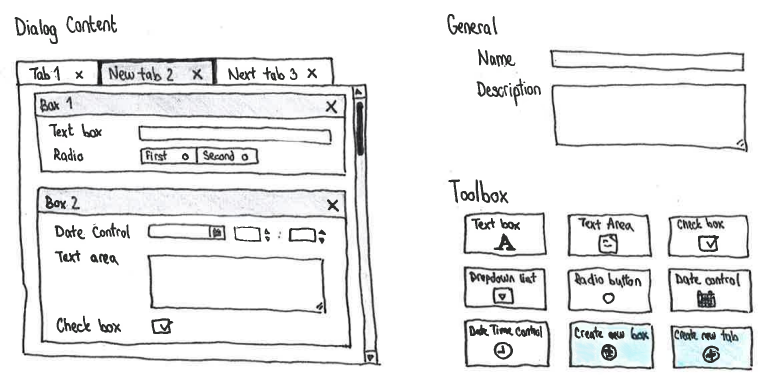
\includegraphics[width=15cm,keepaspectratio]{fig/mockup-3}
  \caption{Mockup of a third version with the buttons moved into the toolbox}
  \label{fig:mockup-3}
\end{figure}

For the Dialog Editor implementation, the version of the design on
Figure~\ref{fig:mockup-2} has been used for the Dialog Editor implementation
so far.

\chapter{Used technologies}\label{ch:technologies}

One of the requirements for the implementation was to use the JavaScript
framework AngularJS. On top of that, to make the implementation easier,
a few extra JavaScript libraries were used in the project.

\section{AngularJS}

AngularJS\,\footnote{\url{https://angularjs.org/}} is an advanced front-end
JavaScript framework released by Google.
It offers a way to build rich front-end experience with cutting-edge
tools quickly and easily~\cite{Angular}.

The decision to use AngularJS library was made by the ManageIQ community.
The plan is to reimplement many parts of the project's user interface
in AngularJS.
Using AngularJS seemed to be an ideal choice for many reasons.
It provides an easier way to create modularized code and allows to write
structured {\it DRY}\,\footnote{Don't repeat yourself} code.
Another reason to use AngularJS is the reaction to a user's interaction with
the editor. The interaction is evaluated completely in the user's browser, so
a server is saved from a lot of unnecessary communication with the
client\,---\,template loading and reevaluation of state after every change
on the jpage.

\subsection{AngularJS version}

The latest stable AngularJS version\,---\,was choosend for the implementation,
even though at the beginning of the work on the Dialog Editor the version~1.4
was used. The reason for this decision was based on an
effort of the ManageIQ project to hold onto the {\it bleeding edge
technology}\,\footnote{the most advanced stage of a technology with risk of
being unreliable}.
To make it possibile to implement the editor in version~1.5, it was,
among other things, also necessary to solve the dependencies for the
new version.
That meant submitting Pull Requests to the different projects' upstreams that
ManageIQ uses.

\newpage

\subsection{Transition to AngularJS~2.0}

It is worth mentioning that AngularJS
version~2.0\,\footnote{\url{https://angular.io/}} which, at the time of
writing this thesis is still in {\it beta} phase, will not be backwards
compatible with previous versions of AngularJS.

AngularJS developers, however, are making an effort to make the transition to
the new version~2.0 as smooth as possible by backporting version~2.0
functionalities to the minor releases of AngularJS~1.
A nice example is the method {\tt component} that was introduced
in version~1.5, as an alternative to the {\tt directive} method used in
previous versions.
The {\tt component} method allows the creating of new HTML elements with
their own JavaScript code\,---\,{\it controller} and HTML template.
The same can be achieved with the {\tt directive} method, but only by using
a soon to be deprecated style.

A lot of guidance for the transition from AngularJS~1 to AngularJS~2, and
even between AngularJS~1 minor versions, can be found on the
internet~\cite{exploringComponent}, making the situation less problematic.
In the following paragraph is well described the reason to keep up with the
latest AngularJS versions:
\blockquote{There are many changes happening, both inside and outside of the
``Angular world''. The best way to be able to transition to Angular~2.0 is to
keep our apps updated as new Angular versions are released. Staying on~1.2
or~1.3 until~2.0 is released is probably going to result in a huge
undertaking~\cite{prepareToAngular}.}

\section{External libraries}\label{ch:libraries}

\subsection{angular-dragdrop}

As the name of the library suggests, this is the key extension that gives the
implemented editor the ability to work with elements by using the
drag\&drop technique.
{\tt angular-dragdrop}\footnote{\url{https://github.com/codef0rmer/angular-dragdrop}}
is a JavaScript library created as an AngularJS wrapper for the jQueryUI
drag\&drop functionalities.
For that reason, some might notice some
familiar attributes in the implemented components that are coming from jQueryUI
and will be described in the following part of this document.

The reasons for choosing this library for the implementation is its
prevalence, that implies a wider support and development.
A further big advantage of this choice is that another planned part of the
Self Service User Interface with drag\&drop support should use this exact
library, however this was not the main reason for the choice, but rather a
coincidence.

\subsection{ui-sortable}

Another important library for the implementation of Dialog Editor that also
happens to be a wrapper on jQueryUI is {\tt ui-sortable} that is developed as
one of a suite of AngularJS directives grouped in a project called
{\it AngularUI}\,\footnote{\url{https://angular-ui.github.io/}}.

This library allows a much more efficient way to implement the sorting of
elements in dialogs, than would be possible by using
just {\tt angular-dragdrop}.

\subsection{angular-bootstrap-switch}

Not as much important as far as the implementation is concerned, the AngularJS
library {\tt angular-bootstrap-switch} is however significant to the
appearance of the project.

It gives the option of using
{\it Bootstrap Switches}\,\footnote{\url{http://www.bootstrap-switch.org/}} with
the AngularJS library.
Bootstrap Switches are basically HTML {\tt input} elements implemented using
the, among front-end developers, well known library
{\it Bootstrap}\,\footnote{\url{https://getbootstrap.com/}}.
The resulting switch gives a pleasant effect, and is also easier to use
compared to a standard HTML check box, thanks to its size.

\chapter{Implementation}\label{ch:implementation}

Before starting with the reimplementation of Dialog Editor, I needed to
create a whole UI state for dialogs in Self Service.

Before the new implementation, the dialogs in Self Service User Interface were
only used in {\it Service Catalog}, but there was no place where Dialogs could
be listed and certainly not edited.

As a first step, a new field had to be added to navigation
menu\,\footnote{\url{https://github.com/ManageIQ/manageiq-ui-self_service/pull/37/commits/e6c9aa1}}.
That meant adding new AngularJS
router\,\footnote{\url{http://angular-ui.github.io/ui-router/site/\#/api/ui.router}}
state, connecting it with the API and making sure that the
data are being loaded, in this case the count of available dialogs.
In this step it was only needed to modify the JavaScript files that were
already in the project.

The next step, after adding a new field {\it My Dialogs} to the navigation
menu, was to add a new list
state\,\footnote{\url{https://github.com/ManageIQ/manageiq-ui-self_service/pull/37/commits/9846a73}},
and connect it with the menu item intended for dialogs.
To enable the possibility to list dialogs, in this step a HTML
template for the list of dialogs had also to be added.
In addition, filtering and sorting of displayed results is in the dialog
list had to be solved. Figure~\ref{fig:dialog-list} shows how the list state
looks like.

When the list state was ready, the next step was to create a dialog detail
state\,\footnote{\url{https://github.com/ManageIQ/manageiq-ui-self_service/pull/37/commits/4efe83e}}.
An example of this can be seen in Figure~\ref{fig:dialog-detail}.
In this state the user can see how a created dialog looks, and has displayed
the most relevant information, like the date when the dialog was created or the
last time it was updated.

After these three steps, everything that was necessary to start work on the
Dialog Editor had almost been done, the last state that had to be added was the
edit state\,\footnote{\url{https://github.com/ManageIQ/manageiq-ui-self_service/pull/37/commits/77297df}},
where the Dialog Editor is placed.

\section{Dialog Editor}

\subsection{Dynamic Tabs}
The first part that was created as a part of the dialog editor was
Dynamic Tabs\,\footnote{\url{https://github.com/ManageIQ/manageiq-ui-self_service/pull/37/commits/4f4fbb6}},
because, as was mentioned previously in Subsection~\ref{sec:service-dialog},
tabs are on the top level of the data structure for the dialog.

The dynamism of the tabs lies in the ability to add new tabs or remove existing
tabs, and also to change the order of existing tabs.

When creating the Dynamic tabs, a major step was to create the AngularJS
component.
The AngularJS component is named {\tt dynamicTabs} in the code, meaning that
this component can be called in HTML by a new element
{\tt <dynamic-tabs></dynamic-tabs>} created by AngularJS.

That would be the basic description of calling the component, but for our case,
the dynamic tabs also need to get data with the dialogs tabs.
For that, another handy feature of AngularJS called data binding is used.

In the code of the created component an HTML attribute can be specified,
through which the data can be passed, in this case named {\tt tabList}.

For a brief demo, the simplified code for the currently described component
looks like the following code:

\begin{lstlisting}
angular.module('app.components')
.component('dynamicTabs', {
  bindings: {
    tabList: '='
 }
})();
\end{lstlisting}

and usage of it in HTML code would look like this:

\begin{lstlisting}
<dynamic-tabs tab-list='dialog_tabs'></dynamic-tabs>
\end{lstlisting}

where {\tt dialog\_tabs} is a JavaScript object containing all the data that
is necessary.

As for manipulating tabs, adding a new tab is handled by a function
in the component controller named {\tt addTab}. It works with the previously
mentioned data object {\tt tabList}.
In the current implementation, the behavior that leads to adding a new tab is:

\begin{enumerate}
  \item set all current tabs as inactive,
  \item create a new object that has the attribute indicating activity set to {\tt true},
  \item push the newly created data object to the {\tt tabList} array.
\end{enumerate}

New tab is always appended to the end.

Behaviour for deleting the tab that is defined in component controller by the
name {\tt deleteTab} is separated into two steps.
Before deleting the tab, it is necessary to check if the deleted tab is
active.
In case where it is active, the activity needs to be passed to another
tab. Because of that there are two cases for deleting an active tab:

\begin{itemize}
  \item If the deleted tab was last, the activity goes to the previous tab.
  \item If the deleted tab has any following tab, the activity goes to the next
        tab in sequence.
\end{itemize}

In a case where a deleted tab is not active, it is not necessary to handle the
situation, and that tab can be removed from the array.

For both adding and deleting tabs the JavaScript utility library
{\it lodash}\,\footnote{\url{https://lodash.com/}} was used; this allows easier
work with arrays or objects in JavaScript, and came in handy even in other
parts of the implementation.

\subsection{Dialog Edit service}

Upon completion of Dynamic tabs it was most essential to clarify how to
work with data using more than just one component, that was necessary for
the implementation of Dialog Editor.

Creating a {\it service} seemed like an ideal option.
To create a {\it service} appeared an ideal option. This AngularJS
feature makes it possible to share the data between all components where it is
needed and update them reflecting the change between all components.

This component is called {\tt DialogEdit}\,\footnote{\url{https://github.com/ManageIQ/manageiq-ui-self_service/pull/37/commits/69e75a4}} in the implementation.
There are two main methods in this service:

\begin{itemize}
  \item method {\tt setData}, which has simple code that takes the data through
        a parameter, and stores them in service variable {\tt data}:
        \begin{lstlisting}
service.setData = function(data) {
  service.data = data;
};
        \end{lstlisting}
  \item method {\tt getData}, is also a simple method that returns data stored
        in {\tt data} variable:
        \begin{lstlisting}
service.getData = function() {
  return service.data;
};
        \end{lstlisting}
\end{itemize}

The third method\,---\,{\tt updatePosition}, does not have much common with
storing data. It is used for updating {\tt position} attribute for objects that
can be sorted in Dialog Editor. Usage of this method will be described in more
detail in a later section of this document.

\subsection{Dialog Dashboard}

Another AngularJS component created for the Dialog Editor is
{\it Dialog Dashboard}\,\footnote{\url{https://github.com/ManageIQ/manageiq-ui-self_service/pull/37/commits/69e75a4}}.
All the content for each dialog tab is displayed inside this component.
Both Boxes and Fields belonging to the Box are rendered
from the template of this component by using the built-in AngularJS directive
{\it ngRepeat}, which makes it possible to write one template that will be
used for each item inside an iterable collection.

The most important methods are, similar to {\it Dynamic Tabs}, the method used
for adding new boxes\,---\,{\tt addBox} and the method for removing
them\,---\,{\tt removeBox}.

\subsection{Dialog Field}

A component that has a major influence on the editor feeling like
{\it WYSIWYG}\,\footnote{What You See Is What You Get} is Dialog
Field\,\footnote{\url{https://github.com/ManageIQ/manageiq-ui-self_service/pull/37/commits/ce782e4}}.
Thanks to this component, the user can immediately recognize which types of
elements are present in Dialog.

The most important part of this component is its template that includes the
HTML code for every element type that can be used in dialog.
It consists of one large HTML file that uses {\it ngSwitch} directive from
AngularJS, which renders an HTML element depending on its condition.

For a better illustration, the simplified code of the template for this
component looks like this:
\begin{lstlisting}
<div ng-switch on="dialogField.fieldData.type">
    <div ng-switch-when="DialogFieldTextBox">
        <!-- HTML code for Text box field -->
    </div>
    <div ng-switch-when="DialogFieldTextAreaBox"> ... </div>
    <div ng-switch-when="DialogFieldCheckBox"> ... </div>
    <!-- etc. -->
</div>
\end{lstlisting}

In Figure~\ref{fig:dialog-mockup}, it can be seen how the previously described
components are integrated together and in Figure~\ref{fig:dialog-edit} there
is an example of how the created dialog looks in reality.

\begin{figure}
  \centering
  \def\svgwidth{\columnwidth}
  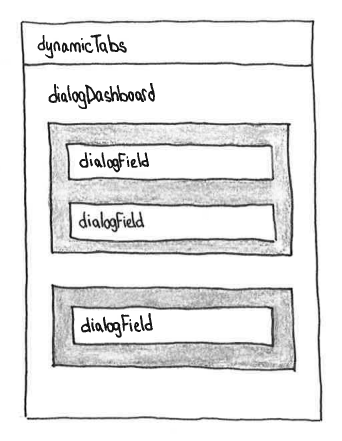
\includegraphics[width=8cm,keepaspectratio]{fig/dialog-mockup}
  \caption{Mockup of a part of the Dialog Editor}\label{fig:dialog-mockup}
\end{figure}

\subsection{Dialog Edit modal}

An important component for editing the details for individual Fields is
{\it Dialog Edit modal}\,\footnote{\url{https://github.com/ManageIQ/manageiq-ui-self_service/pull/37/commits/ce782e4}}.
For every element type, a template through which the user can access
and modify the attributes of dialog field is created.

The {\it Dynamic} is ratger specific. It replaces the original attributes
of the element with attributes specific for dynamic elements. This was
introduced for every element in ManageIQ release {\it Botvinnik}.

The described templates are rendered using the AngularJS function
{\tt directive}, as features of the {\tt component} method do not support
a way to render a different template according to a parameter.

Here is a simplified {\it directive} code, where it is possible to see how the
directive decides which template file is supposed to be rendered, according to
the parameter that is sent by the attribute {\tt template}:
\\
\begin{lstlisting}
.directive('dialogModalTemplate', function() {
  return {
    templateUrl: function(tElement, tAttrs) {
      return 'app/components/dialog-modal-template/' + tAttrs.template;
    },
    scope: true,
  };
});
\end{lstlisting}

For example, a Text area is then rendered from HTML using this directive by
this element:

\begin{lstlisting}
<dialog-modal-template ng-switch-when="DialogFieldTextAreaBox"
                       template="edit-dialog-modal-text-area-box.html">
\end{lstlisting}

Figure~\ref{fig:dialog-modal} is showing how a modal looks for the Radio
button field.

\subsection{Draggable components}

The last component that was
created\,\footnote{\url{https://github.com/ManageIQ/manageiq-ui-self_service/pull/37/commits/036eef6}}
for the implementation works more or less
as a placeholder for new Fields that can be dragged to the Dialog Box.

In the controller all the necessary attributes for all types of
elements are described, so after dragging the element to the box, the user can
immediately see, how the element will approximately look like.

\subsection{Drag\&Drop and sorting}

To allow the user to manipulate objects of the dialog easier than it was in
the previous implementation, a mouse is used in the editor for sorting and
dragging elements.

As was mentioned in the chapter describing the {\it ui-sortable} library, it
offers a very efficient way of implementing the sorting of elements.

For the element, where the sorting should be applied, the {\it ngModel}
directive is specified, through which data are provided to the library.
The data contains an array that is connected with rendered elements, and after
changing the position of the element by dragging it to a different place, the
position of the element in the array is changed as well.

The definition of the component may even specify the sorting behaviour that
jQueryUI offers.

In the implementation, sorting is used for Tabs, Boxes and Dialog Fields.
On the other hand, dragging elements is used only for one component\,---\,the
draggable components that were described in the previous sub-section.
The droppable zone for these elements is the Dialog Dashboard, that also has an
object in its component's code, where behaviour is specified, again by
using jQueryUI possible interactions.

\chapter{Effectivity and Users comfort}\label{ch:effectivity}

One of the most important goals of this thesis was to improve the effectivity
and the users comfort.
The main difference in terms of effectivity can be observed on the amount of
the data transfered between the server and client, that is significantly
lowered by using the new version of the Dialog Editor.

For a better illustration a new dialog was created while observing data flow
using the network diagnostic tool Wireshark.

In both cases the created dialog had the same content. It contained only one
element\,---\,Check Box.

In Figure~\ref{fig:0-rails-add-new-checkbox-src-dst-tcp} you can see the
size of TCP packets transfered between the client and the server in a process
of creating the new dialog by using the older version of Dialog Editor in the
ManageIQ Admin and Operations User Interface.
The summarized stats are displayed in Table~\ref{tab:0-rails-add-new-checkbox-src-dst-tcp}.

\vspace{\baselineskip}
\noindent\begin{minipage}{\linewidth}
  \centering
  \begin{tabular}{|l|l|}
    \hline
    {\bf Packets}             & 94         \\ \hline
    {\bf Bytes}               & 154290     \\ \hline
    {\bf Average packet size} & 1641 bytes \\ \hline
  \end{tabular}
  \captionof{table}{Summary of the TCP data flow between client and server by using the old version of Dialog Editor}
  \label{tab:0-rails-add-new-checkbox-src-dst-tcp}
  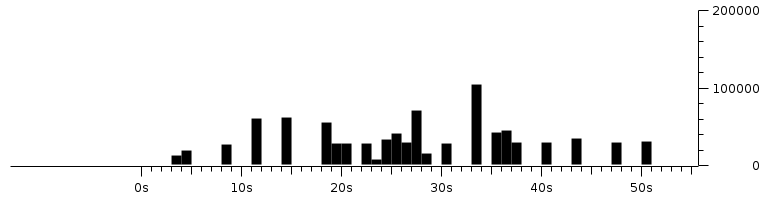
\includegraphics[width=15cm,keepaspectratio]{fig/0-rails-add-new-checkbox-src-dst-tcp}
  \captionof{figure}{Sizes of TCP packets transfered between client and server by using the old version of Dialog Editor}
  \label{fig:0-rails-add-new-checkbox-src-dst-tcp}
\end{minipage}
\vspace{\baselineskip}

In the case where the new Dialog Editor was used, as can be seen from the
Table~\ref{tab:1-ssui-add-new-checkbox-src-dst-tcp}, the amount of transfered
data was more than $10\times$ lower.

\vspace{\baselineskip}
\noindent\begin{minipage}{\linewidth}
  \centering
  \begin{tabular}{|l|l|}
    \hline
    {\bf Packets}             & 81        \\ \hline
    {\bf Bytes}               & 13479     \\ \hline
    {\bf Average packet size} & 166 bytes \\ \hline
  \end{tabular}
  \captionof{table}{Summary of the TCP data flow between client and server by using the new version of Dialog Editor}
  \label{tab:1-ssui-add-new-checkbox-src-dst-tcp}
  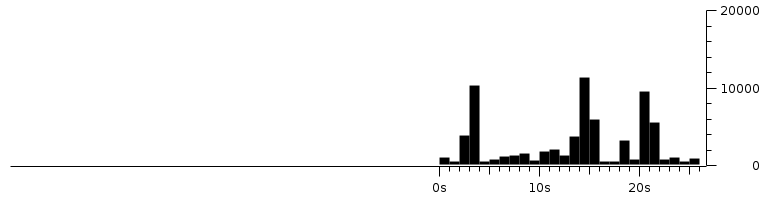
\includegraphics[width=15cm,keepaspectratio]{fig/1-ssui-add-new-checkbox-src-dst-tcp}
  \captionof{figure}{Sizes of TCP packets transfered between client and server by using the new version of Dialog Editor}
  \label{fig:1-ssui-add-new-checkbox-src-dst-tcp}
\end{minipage}
\vspace{\baselineskip}

As for memcached, from the graph in
Figure~\ref{fig:0-rails-add-new-checkbox-memcached} it can be told, that the
amount of data used by memcached is almost the same as the amount of data
transfered by the TCP communication between client and server. On the other
hand, by using the new Dialog Editor, memcached is only used for storing the
session token. As you can see in
Figure~\ref{fig:1-ssui-add-new-checkbox-memcached}, the communication with
memcached has occured only once.

\vspace{\baselineskip}
\noindent\begin{minipage}{\linewidth}
  \centering
  \begin{tabular}{|l|l|}
    \hline
    {\bf Packets}             & 126        \\ \hline
    {\bf Bytes}               & 645948     \\ \hline
    {\bf Average packet size} & 5127 bytes \\ \hline
  \end{tabular}
  \captionof{table}{Summary of transmitted memcached data by using the old version of Dialog Editor}
  \label{tab:0-rails-add-new-checkbox-memcached}
  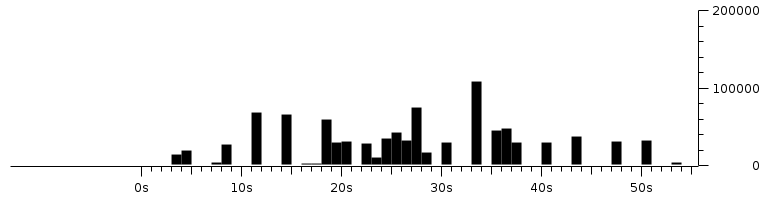
\includegraphics[width=15cm,keepaspectratio]{fig/0-rails-add-new-checkbox-memcached}
  \captionof{figure}{Sizes of memcached packets transfered by using the old version of Dialog Editor}
  \label{fig:0-rails-add-new-checkbox-memcached}
\end{minipage}
\vspace{\baselineskip}

\vspace{\baselineskip}
\noindent\begin{minipage}{\linewidth}
  \centering
  \begin{tabular}{|l|l|}
    \hline
    {\bf Packets}             & 14        \\ \hline
    {\bf Bytes}               & 2295      \\ \hline
    {\bf Average packet size} & 164 bytes \\ \hline
  \end{tabular}
  \captionof{table}{Summary of transmitted memcached data by using the new version of Dialog Editor}
  \label{tab:1-ssui-add-new-checkbox-memcached}
  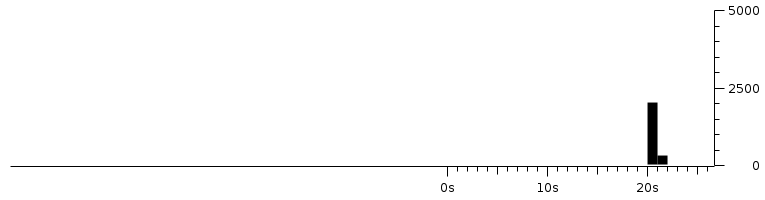
\includegraphics[width=15cm,keepaspectratio]{fig/1-ssui-add-new-checkbox-memcached}
  \captionof{figure}{Sizes of memcached packets transfered by using the new version of Dialog Editor}
  \label{fig:1-ssui-add-new-checkbox-memcached}
\end{minipage}
\vspace{\baselineskip}

As was mentioned at the beginning of the document, the current
implementation forces the user to spend an uncomfortably long amount of time in
the editor. By giving the user a way to create the dialog by using a drag\&drop
technique, the workflow of creating a new dialog is much smoother.

As an example we can take the graphs comparing an amount of the data
transmitted between the client and the server.
Comparing the time axes these, we can see, that the length of the time that was
spent by creating the dialog containing one Check box is approximately
$2\times$ shorter while using the new version of the dialog editor.

\chapter{Conclusion}\label{ch:conclusion}

In my work on the Dialog Editor I have learned to use the AngularJS framework
and studied the original version of the Dialog Editor.
The gained knowledge allowed me to to implement the new interactive editor for
ManageIQ with drag\&drop technique together with specs coverage.
In this document I've summarized the solution and effectivity of the previous
and the new implementation.

One of the biggest advantages of the implementation is that the whole work is
created as an open source project that will be used in the future as a separate
component, allowing many developers to improve or modify the Dialog Editor for
their own purposes.

The result of the work is Dialog Editor that has been introduced as a Pull
Request to the project's
upstream~\footnote{\url{https://github.com/ManageIQ/manageiq-ui-self_service/pull/37}}.
At this moment the work is in review status by the members of the Red Hat
CloudForms team.

\section{Ideas for a future development}

Even though the goal set by the bachelor thesis was successfuly achieved,
a lot of work can still be done in the Dialog Editor to improve the user's
experience.

Removing the tabs, boxes and elements is not protected by any confirmation.
Especially in the case of tab removal, this could lead to the unwanted
situation, when the user would accidentaly remove a part of the dialog.
On the other hand, requesting an answer from the user every time he wants to
remove a part of the dialog would be uncomfortable from the user's perspective.
The better way would be to give the user an option to undo the changes.
To achieve this solution, using the {\tt sessionStorage} from
the Web Storage API\,\footnote{\url{https://developer.mozilla.org/en-US/docs/Web/API/Web_Storage_API}}
seems to be the best option.

Another improvement could be done in the drag\&drop toolbox zone.
In the current solution, the element dropped to the dialog's box is always
appended at the end of all elements in the box.
A more comfortable solution would be to detect where exactly the user has
dropped the element, and insert it at the position it was dropped at.
Another problem is with sorting elements in the box. Right now it is only
possible to sort the elements inside of one box, but not between boxes.

Purely esthetical change, but still related to the drag\&drop is the idea to
provide a visual suggestion for every draggable element. At the first sight it
may not be clear to the users which parts of the Dialog Editor are draggable,
and where they can be dropped.

As was mentioned earlier in Chapter~\ref{ch:design}, an
option to move buttons for creating a new tab and box from the area where the
dialog is displayed into the toolbox of draggable elements is also discussed.

The suggestions for the improvements mentioned above will be discussed with
the Red Hat UX Design and the CloudForms teams to provide the best possible
solution.
